
\section{Motivations}

Over the last three decades, Computational Fluid Dynamics (CFD) simulations have become commonplace as a tool in the engineering and design of high-speed aircraft.  Wind tunnel experiments are often complemented by computational simulations, and CFD technologies have proved very useful in both the reduction of aircraft development cycles and the simulation of experimentally difficult conditions.  Great advances have been made in the field since its introduction, especially in areas of meshing, computer architecture, and solution strategies.  Despite this, there still exist many computational limitations in existing CFD methods:  
\begin{itemize}
\item \textbf{Higher order methods :} Higher order methods stand to offer large computational savings through a more efficient use of discrete degrees of freedom.  However, there are very few working higher-order CFD codes in existence, and most higher order methods tend to degrade to first-order accuracy near shocks. The use of higher order codes to solve the steady state equations is even rarer, where convergence of discrete nonlinear steady equations is a tricky issue \cite{BoeingHigherOrder}.  
\item \textbf{Automatic adaptivity :} The use of adaptive meshes is crucial to many CFD applications, where the solution can exhibit very localized sharp gradients and shocks.  Good resolution for such problems under uniform meshes is computationally prohibitive and impractical for most physical regimes of interest.  However, the construction of ``good" meshes is a difficult task, usually requiring a-priori knowledge of the form of the solution \cite{andersonCFDBook}.  An alternative set of strategies are automatically adaptive schemes; such methods usually begin with a coarse mesh and refine based on the minimization of some error.  However, this task is difficult, as the convergence of numerical methods for problems in CFD is notoriously sensitive to mesh quality.  Additionally, the use of adaptivity becomes even more difficult in the context of higher order and $hp$ methods \cite{BoeingHigherOrder}.  
\end{itemize}
Both of these issues are tied to the notion of \emph{robustness}.  We define robustness loosely as the degradation of the quality of numerical solutions with respect to a given problem parameter.  In the context of CFD simulations, the parameter of interest is the Reynolds number (the nondimensional equivalent of the inverse of the viscosity) --- for typical physical conditions of interest for the compressible Navier-Stokes equations, the Reynolds number is extremely high, on the order of 1e7, yielding solutions with two vastly different scales - inviscid phenomena at an $O(1)$ scale, and $O(1e-7)$ viscous phenomena.  

The full Navier-Stokes equations are not well understood in a mathematical sense --- in order to more clearly illustrate the issue of robustness for problems in CFD, we will study first the important model problem of convection-dominated diffusion.  

\subsection{Singular perturbation problems and robustness}

%Historically, the Galerkin method has been very successfully applied to a broad range of problems in solid mechanics, for which the variational problems resulting from the PDE are symmetric and coercive (positive-definite). It is well known that the finite element method produces optimal or near-optimal results for such problems, with the finite element solution matching or coming close to the best approximation of the solution in the finite element space. However, 

Standard numerical methods tend to perform poorly across the board for the class of PDEs known as singular perturbation problems; these problems are often characterized by a parameter that may be either very small or very large.  An additional complication of singular perturbation problems is that very often, in the limiting case of the parameter blowing up or decreasing to zero, the PDE itself will change types (e.g.\ from elliptic to hyperbolic).  A canonical example of a singularly perturbed problem is the convection-diffusion equation in domain $\Omega \subset \mathbb{R}^3$,
\[
\div \left(\beta u\right) - \epsilon \Delta u = f.
\]
The equation models the steady-state distribution of the scalar quantity $u$, representing the concentration of a quantity in a given medium, taking into account both convective and diffusive effects. Vector $\beta \in \mathbb{R}^3$ specifies the direction and magnitude of convection, while the singular perturbation parameter $\epsilon$ represents the diffusivity of the medium. In the limit of an inviscid medium as $\epsilon\rightarrow 0$, the equation changes types, from elliptic to hyperbolic, and from second order to first order.

We will illustrate the issues associated with numerical methods for this equation using one dimensional examples.  In 1D, the convection-diffusion equation is
\begin{align*}
\beta u'-\epsilon u'' &= f.
\end{align*}
For Dirichlet boundary conditions $u(0)=u_0$ and $u(1)= u_1$, the solution can develop sharp boundary layers of width $\epsilon$ near the outflow boundary $x=1$. 

\begin{figure}[!h]
\centering
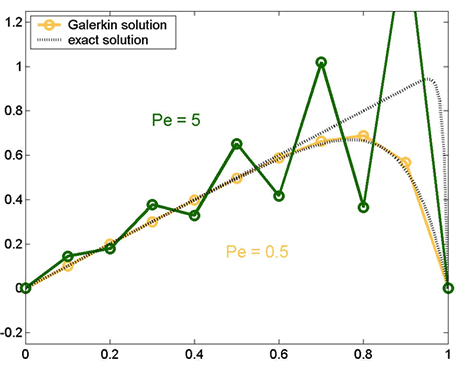
\includegraphics[scale=.5]{figs/GalerkinOscTight.png}
\caption{Oscillations in the 1D finite element solution of the convection-diffusion equation for small diffusion \cite{GalerkinOsc}. Standard finite volume and finite difference methods exhibit similar behavior.}
\label{fig:GalerkinOsc}
\end{figure}
We consider for now the Galerkin finite element method as applied to convection-dominated diffusion.  Standard finite element methods (as well as standard finite volume and finite difference methods) perform poorly for the case of small $\epsilon$.  The poor performance of the finite element method for this problem is reflected in the bound on the error in the finite element solution --- under the standard Bubnov-Galerkin method with $u\in H^1(0,1)$, we have the bound given in \cite{roos2008robust}:
\[
\|u-u_h\|_\epsilon \leq C \inf_{w_h}\|u-w_h\|_{H^1(0,1)},
\]
for $\|u\|_\epsilon^2 \coloneqq \|u\|_{L^2}^2 + \epsilon \|u'\|_{L^2}^2$, with $C$ independent of $\epsilon$. An alternative formulation of the above bound is 
\[
\|u-u_h\|_{H^1(0,1)} \leq C(\epsilon) \inf_{w_h}\|u-w_h\|_{H^1(0,1)},
\]
where $C(\epsilon)$ grows as $\epsilon\rightarrow 0$. The dependence of the constant $C$ on $\epsilon$ is what we refer to as a \textit{loss of robustness} --- as the singular perturbation parameter $\epsilon$ decreases, our finite element error is bounded more and more loosely by the best approximation error.  As a consequence, the finite element solution can diverge significantly from the best finite element approximation of the solution for very small values of $\epsilon$.  For example, Figure~\ref{fig:GalerkinOsc} shows an example of how, on a coarse mesh, and for small values of $\epsilon$, the Galerkin approximation of the solution to the convection-diffusion equation with a boundary layer develops spurious oscillations everywhere in the domain, even where the best approximation error is small.  These oscillations grow in magnitude as $\epsilon \rightarrow 0$, eventually polluting the entire solution.\footnote{For nonlinear shock problems, the solution often exhibits sharp gradients or discontinuities, around which the solution would develop spurious Gibbs-type oscillations. These are a result of underresolution of the solution, and are separate from the oscillations resulting from a lack of robustness.}

\section{Goal}

From the perspective of the full Navier-Stokes equations, this loss of robustness is doubly problematic.  Not only will any nonlinear solution suffer from similar non-physical oscillations, but nonlinear solvers themselves may fail to yield a solution due to such instabilities.  A nonlinear solution is almost always computed by solving a series of linear problems whose solutions will converge to the nonlinear solution under appropriate assumptions, and the presence of such oscillations in each linear problem can cause the solution convergence to slow significantly or even diverge.  

Our aim is to develop a \emph{stable, higher order adaptive scheme} for the steady compressible laminar Navier-Stokes equations in transonic/supersonic regimes that is \emph{robust for very small viscosity}.  In particular, we hope to present a method for which $hp$-adaptivity can be applied to problems in compressible flow.  The goal of this dissertation will be to develop a mathematical theory demonstrating the robustness in $\epsilon$ of our method for singularly perturbed convection-diffusion problems, and to demonstrate its feasibility as a CFD solver by applying it to several benchmark problems.  

\section{Literature review}

For the past half-century, problems in CFD have been solved using a multitude of methods, many of which are physically motivated, and thus applicable only to a small number of problems and geometries. We consider more general methods, whose framework is applicable to a larger set of problems; however, our specific focus will be on the problems of compressible aerodynamics involving small-scale viscous phenomena (i.e.\ boundary layers and, if present, shock waves). Broadly speaking, the most popular general methods include (in historical order) finite difference methods, finite volume methods, and finite element methods.  

\subsection{Finite difference and finite volume methods}

For linear problems, finite difference (FD) methods approximate derivatives based on interpolation of pointwise values of a function.  In the context of conservation laws, FD methods were popularized first by Lax, who introduced the concepts of the monotone scheme and numerical flux. For the conservation laws governing compressible aerodynamics, FD methods approximate the conservation law, using some numerical flux to reconstruct approximations to the derivative at a point. Finite volume (FV) methods are similar to finite difference methods, but approximate the integral version of a conservation law as opposed to the differential form. FD and FV have roughly the same computational cost/complexity; however, the advantage of FV methods over FD is that FV methods can be used on a much larger class of problems and geometries than FD methods, which require uniform or smooth structured meshes. 

Several ideas were introduced to deal with oscillations in the solution near a sharp gradient or shock: artificial diffusion, total variation diminishing (TVD) schemes, and slope limiters. However, each method had its drawback, either in terms of loss of accuracy, dimensional limitations, or problem-specific parameters to be tuned \cite{Shu:Lectures}. Harten, Enquist, Osher and Chakravarthy introduced the essentially non-oscillatory (ENO) scheme in 1987 \cite{ENO}, which was improved upon with the weighted essentially non-oscillatory (WENO) scheme in \cite{WENO}. WENO remains a popular choice today for both finite volume and finite difference schemes. Most of these methods can be interpreted as adding some specific artificial diffusion to the given numerical scheme.  We refer to such schemes as \emph{modified equation} methods, as the exact solution no longer satisfies the discrete system due to the presence of additional artificial diffusion terms.  

Historically, finite volumes and finite difference methods have been the numerical discretizations of choice for CFD applications; the simplicity of implementation of the finite difference method allows for quick turnaround time, and the finite volume method is appealing due to its locally conservative nature and flexibility. More recently, the finite element (FE) method has gained popularity as a discretization method for CFD applications for its stability properties and rigorous mathematical foundations. Early pioneers of the finite element method for CFD included Zienkiewicz, Oden, Karniadakis, and Hughes \cite{ChungCFDBook}.  

\subsection{Stabilized finite element methods}

The finite element/Galerkin method has been widely utilized in engineering to solve partial differential equations governing the behavior of physical phenomena in engineering problems.  The method relates the solution of a partial differential equation (PDE) to the solution of a corresponding variational problem. The finite element method itself provides several advantages --- a framework for systematic mathematical analysis of the behavior of the method, weaker regularity constraints on the solution than implied by the strong form of the equations, and applicability to very general physical domains and geometries for arbitrary orders of approximation. 

Historically, the Galerkin method has been very successfully applied to a broad range of problems in solid mechanics, for which the variational problems resulting from the PDE are often symmetric and coercive (positive-definite). It is well known that the finite element method produces optimal or near-optimal results for such problems, with the finite element solution matching or coming close to the best approximation of the solution in the finite element space. However, standard Galerkin methods tend to perform poorly for singular perturbation problems, developing instabilities when the singular perturbation parameter is very small. 

Traditionally, instability/loss of robustness in finite element methods has been dealt with using residual-based stabilization techniques.  Given some variational form, the problem is modified by adding to the bilinear form the strong form of the residual, weighted by a test function and scaled by a stabilization constant $\tau$.  The most well-known example of this technique is the streamline-upwind Petrov-Galerkin (SUPG) method, which is a stabilized FE method for solving the convection-diffusion equation using piecewise linear continuous finite elements \cite{SUPG}.  SUPG stabilization not only removes the spurious oscillations from the finite element solution of the convection-diffusion equation, but delivers the best finite element approximation in the $H^1$ norm in 1D.  

\subsubsection{SUPG}

All Galerkin methods involve both trial (approximating) and test (weighting) functions.   Standard Galerkin methods, where these trial and test functions are taken from the same space, are referred to as Bubnov-Galerkin methods.  Petrov-Galerkin methods refer most often to methods where test and trial functions \emph{differ}, leading to differing test and trial spaces.\footnote{Hughes takes the more general definition of a Petrov-Galerkin method to be any Galerkin method other than a classical Bubnov-Galerkin method.}  The Streamline Upwind Petrov Galerkin (SUPG) method is a stabilization method for $H^1$-conforming finite elements, the idea of which was originally motivated by artificial diffusion techniques in finite differences.  In particular, for the homogeneous 1D convection-diffusion equation, it is possible to recover, under a finite difference method, the exact solution at nodal points by adding an ``exact" artificial diffusion based on the mesh size $h$ and the magnitudes of the convection $\beta$ and the viscosity $\epsilon$.  The idea of ``exact" artificial viscosity was adapted to finite elements not through the direct modification of the equations, but through the \emph{test} functions and weighting of the residual. \footnote{Finite element and Galerkin methods are often referred to as ``weighted residual" methods, since the starting point of both is to multiply the residual by a particular test, or weighting, function.  Standard Bubnov-Galerkin methods simply choose these weighting functions to be the same as the the basis functions used to approximate the solution.  }

We will introduce the SUPG method at the abstract level for illustrative purposes only.  Further details and perspectives on the SUPG method can be found in \cite{SUPG}, as well as in an upcoming book by Hughes.  The convection-diffusion equation can be written as follows:
\[
Lu = \left(L_{\rm adv} + L_{\rm diff} \right) u = f,
\]
where $L_{\rm adv}u \coloneqq \div \left(\beta u\right)$ is the first order advective operator, and $L_{\rm diff}u \coloneqq \epsilon \Delta u$ is the second-order diffusive operator.  Let us assume $u$ to be a linear combination of piecewise-linear basis functions $\phi_i, i = 0,\ldots,N$ (then, within each element, $L_{\rm diff} u = 0$).  If $b(u,v)$ and $l(v)$ are the bilinear form and load for the standard Galerkin method (resulting from multiplying by a test function $v$ and integrating both convective and diffusion terms by parts), the SUPG method is then to solve $b_{\rm SUPG}(u,v) = l_{\rm SUPG}(v)$, where $b_{\rm SUPG}(u,v)$ and $l_{\rm SUPG}(v)$ are defined as
\begin{align*}
b_{\rm SUPG}(u,v) &= b(u,v)+ \sum_{K} \int_{K} \tau \LRp{L_{\rm adv} v} \LRp{L u - f} \\
l_{\rm SUPG}(v) &= l(v) + \sum_{K} \int_{K} \tau \LRp{L_{\rm adv}v} f
\end{align*}
for where $\tau$ is the SUPG parameter. For uniform meshes in 1D, $\tau$ is chosen such that, for $f=0$, the matrix system resulting from SUPG is exactly equal to the finite difference system under ``exact" artificial diffusion.  However, unlike exact artificial diffusion, for $f\neq 0$, the SUPG method still delivers optimal stabilization.  In fact, the SUPG finite element solution in 1D is nothing less than the nodal interpolant and the best $H^1_0$ approximation of the exact solution, as seen in Figure~\ref{fig:SUPG}.

\begin{figure}[!h]
\centering
\subfigure[SUPG and standard FEM solutions]{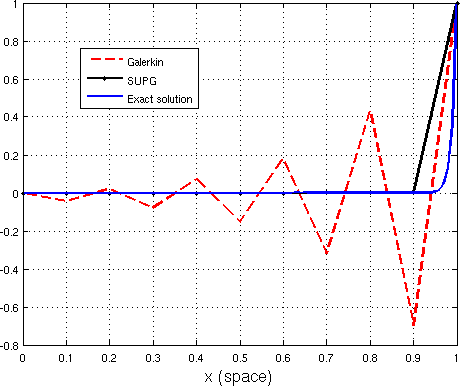
\includegraphics[scale=.475]{figs/SUPG.png}}
\subfigure[SUPG test function]{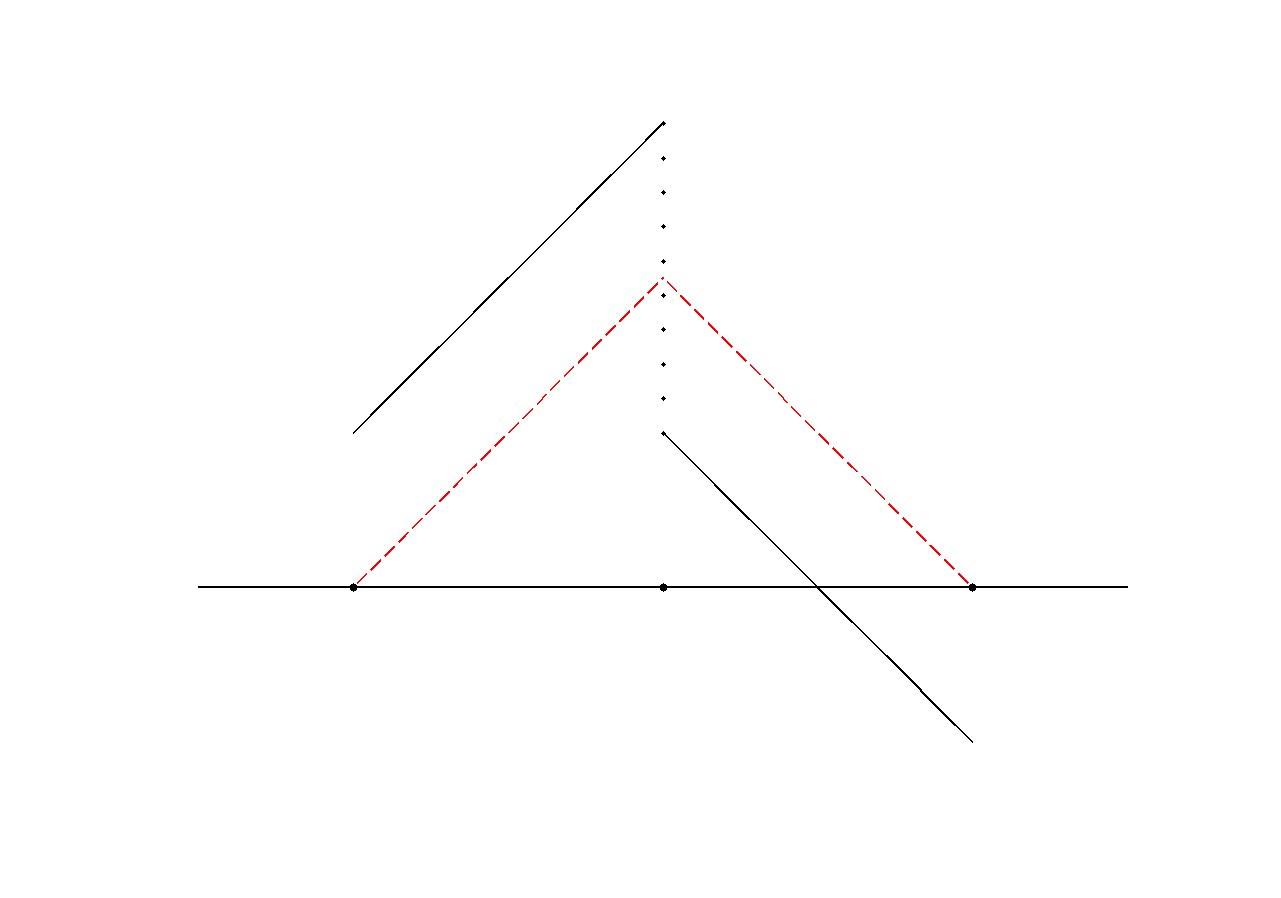
\includegraphics[scale=.25]{figs/SUPGtest.png}}
\caption{SUPG and standard Bubnov-Galerkin solutions to the 1D convection-dominated diffusion equation, and a modified SUPG test function (in black) corresponding to a linear basis ``hat" function (in red).  The upwind portion of the element is emphasized, while the downwind portion is decreased.  The magnitude of the discontinuity between the upwind and downwind portion is controlled by the intrinsic timescale parameter $\tau$. }
\label{fig:SUPG}
\end{figure}

The idea of emphasizing the upwind portion of a test function is an older idea, introduced in 1977 by Zienkiewicz et al.\ in \cite{zienkUpwind}.  However, the precise amount of upwinding,\footnote{Insufficient upwinding results in a method which still exhibits oscillations and instabilities, while excessive upwinding leads to an overly diffusive method.} as well as the connection to residual-based stabilization methods, were novel to SUPG.  

For appropriately chosen $\tau$, the method can be generalized for higher order elements as well.  In higher dimensions, and the SUPG solution is very close to, but no longer the $H^1_0$ best approximation for 2D and 3D problems \cite{HughesSangalliSUPG}.  Since its inception, SUPG is and has been the most popular stabilization method of choice for convection-diffusion type problems, in both academic and industry applications. 

An important feature of SUPG and other residual-based stabilization techniques that separates it from modified equation methods is the idea of \textit{consistency} --- by adding stabilization terms based on the residual, the exact solution still satisfies the same variational problem (i.e.\ Galerkin orthogonality still holds). Contrast this to the artificial diffusion methods in finite difference and finite volume methods, where a specific amount of additional viscosity is added based on the magnitude of the convection and diffusion parameters: unlike residual-based stabilization schemes, the exact solution to the original equation no longer satisfies the new stabilized formulation.  

This addition of residual-based stabilization terms can be interpreted as a modification of the test functions as well.  For SUPG, the formulation can equivalently be written as
\[
b\LRp{u,\tilde{v}_{i}} = l\LRp{\tilde{v}_{i}}, \quad \forall i = 1,\ldots,N-1
\]
where the SUPG test function $\tilde{v}_{i}$ is defined elementwise as
\[
\tilde{v}_{i} = \phi_i(x) + \tau L_{\rm adv} \phi_i.  
\]
In other words, the test functions $\tilde{v}_{i}$ is a perturbation of the basis function $\phi_i$ by a scaled advective operator applied to $\phi_i$.  For a linear $C^0$ basis function (the ``hat" function), this naturally leads to a bias in the upwind or streamline direction of the flow $\beta$, as seen in Figure~\ref{fig:SUPG}.  

An important connection can now be made --- stabilization can be achieved by changing the test space for a given problem.  We will discuss in Section~\secref{optimalTest} approaching the idea of stabilization through the construction of \textit{optimal test functions} to achieve optimal approximation properties. 

\subsubsection{DG methods}

Discontinuous Galerkin (DG) methods form a subclass of FEM; first introduced by Reed and Hill in \cite{Reed:73}. These methods were later analyzed Raviart et al \cite{DGRaviart} and later by Johnson et al \cite{DGJohnson}, who contributed a mathematical analysis of the original method of Reed and Hill, as well as by Cockburn and Shu \cite{CockburnShu:DG}, who solved the Euler equations by applying concept of Lax's numerical flux within the context of DG.

Advantages of DG methods include the local conservation property, easily modified local orders of approximation, ease of adaptivity in both $h$ and $p$, and efficient parallelizability. Rather than having a continuous basis where the basis function support spans multiple element cells, DG opts instead for a discontinuous, piecewise polynomial basis, where, like FV schemes, a \emph{numerical flux} facilitates communication between neighboring elements (unlike FV methods, however, there is no need for a reconstruction step). 

The formal definition of the numerical flux (attributed to Peter Lax) on an element boundary is some function of the values on the edges of both the neighboring elements.  An additional reason for the popularity of DG methods is that they can be interpreted as stabilized FE methods (and vice versa) through appropriate choices of this numerical flux \cite{Brezzi20063293}. We will illustrate this with the steady convection equation in 1D:
\begin{align*}
\pd{\left(\beta(x) u\right)}{x} = f, \quad u(0) &= u_0.
\end{align*}
The DG formulation is derived by multiplying by a test function $v$ with support only on a single element $K = [x_K,x_{K+1}]$ and integrating by parts. The boundary term is left alone, such that the local formulation is 
\[
\left.\beta u v\right|_{x_K}^{x_{K+1}} + \int_K -\beta u \pd{v}{x} = \int_K f v,
\]
and the global formulation is recovered by summing up all element-wise local formulations. However, the boundary term in the local formulation is presently ill-defined, as both $u$ and $v$ are dual-valued over element boundaries. Consequently, we make the choice to define the values of $u$ on the boundary (the \emph{traces} of $u$) as
\begin{align*}
u(x_K) \coloneqq u(x_K^-), \quad u(x_{K+1}) \coloneqq u(x_{K+1}^-),
\end{align*}
where $u(x_K^-)$ is the value of $u$ at $x_K$ as seen from the left, and $u(x_K^+)$ the value as seen from the right. Similarly, the traces of $v$ are defined to be
\begin{align*}
v(x_K) \coloneqq v(x_K^+), \quad v(x_{K+1}) \coloneqq v(x_{K+1}^-),
\end{align*}
For $\beta$ positive, $v(x_K^+)$ is the \emph{upwind} value of $v(x_K)$, and we refer to DG under this specific choice of traces as upwind DG.  This specific choice of $v(x_K)$ as the upwind value is crucial; similarly to SUPG, the upwind DG emphasizes the test function in the direction of convection and changes the way the residual is measured.  As it turns out, the performance of DG for convection-type problems is closely tied to this upwinding --- choosing the value of $v(x_K)$ to be the downwind value $v(x_K^-)$ leads to an unstable method, while choosing $v(x_K)$ to be the average of the upwind and downwind values leads to a DG method with suboptimal stability properties, similar to an $H^1$-conforming continuous Galerkin approximation\cite{Brezzi20063293}.\footnote{For second-order convection-diffusion problems with small diffusion, the additional regularity imparted by choice of the DG numerical flux is often insufficient, and SUPG-type stabilization is also applied.}

Another perspective on the use of the numerical flux in DG methods is that the selection of specific DG fluxes imparts \emph{additional regularity} where needed.  For example, for the pure convection problem, the solution has a distributional derivative in the streamline direction, but is only $L^2$ in the crosswind direction. As a consequence of the regularity of the solution, the boundary trace of the solution is defined only in the direction of convection. The upwind DG method addresses the above issue by choosing the numerical flux to be the upwind flux; in this case, the DG numerical flux can be viewed as imparting additional regularity to the discrete solution than is implied by the continuous setting \cite{DPG1,DPG3}.  

\subsubsection{HDG}

A more recent development in DG methods is the idea of \emph{hybridized} DG (HDG), introduced by Cockburn, Gopalakrishnan and Lazarov \cite{hybridDG}. The hybridized DG framework identifies degrees of freedom with support only on element edges, which can be interpreted as Lagrange multipliers enforcing weak continuity of the trial space. HDG methods treat numerical \emph{traces} and numerical \emph{fluxes} differently depending on the form of the boundary term resulting from integration by parts. The numerical trace (the result of integrating by parts the gradient) in HDG methods is chosen to be an unknown, while the numerical flux (the result of integrating by parts the divergence) is chosen to be an appropriate function of both function values on neighboring elements and the numerical trace. 

By a careful choice of the numerical flux, the global HDG formulation can be reduced to a single equation involving only the numerical trace degrees of freedom, referred to as the \emph{global} problem. Once the global problem is solved, interior degrees of freedom can be recovered in parallel through so-called \emph{local} problems \cite{HDGprojection}. 

HDG methods are an active topic of current research, since they address several criticisms of common DG methods (large number of globally coupled degrees of freedom, complicated/inefficient implementation procedures, suboptimal convergence of approximate fluxes). Note that HDG methods still fall under the category of stabilized methods --- stabilization techniques are employed through the choice of the HDG numerical flux, which involves some stabilization parameter $\tau$. 

\section{Scope}

This dissertation will proceed in four main parts.  We will begin by introducing the abstract Discontinuous Petrov-Galerkin (DPG) method as a minimum residual method for linear problems and highlighting some important properties of the method.  Our next step will be to formulate and prove the robustness of a DPG method (with respect to $\epsilon$) for the model problem of convection-dominated diffusion.  Finally, we will extend and apply the DPG method to singularly perturbed nonlinear problems in CFD, presenting results for the Burgers and compressible Navier-Stokes equations.  

